\section*{Materials and Methods}
\label{sec:methods}

This section defines the common graph-classification setting, the CR-GNN architecture family, the benchmark package, and the shared experimental protocol. The goal is to isolate where information is reused while keeping the remaining pipeline as consistent as possible.

\subsection*{Problem definition and notation}

Let $\mathcal{G} = (\mathcal{V}, \mathcal{E})$ denote an undirected or directed graph, where $\mathcal{V} = \{v_1, v_2, \ldots, v_n\}$ is the set of $n$ nodes and $\mathcal{E} \subseteq \mathcal{V} \times \mathcal{V}$ is the set of edges. Each node $v_i \in \mathcal{V}$ is associated with a feature vector $\mathbf{x}_i \in \mathbb{R}^{d_{\text{in}}}$, and the node features for the entire graph are collected in $\mathbf{X} \in \mathbb{R}^{n \times d_{\text{in}}}$. The graph structure is represented using an adjacency matrix $\mathbf{A}$.

Given a training dataset $\mathcal{D} = \{(\mathcal{G}_i, y_i)\}_{i=1}^{N}$, the objective is to learn a mapping function $f_\theta: \mathcal{G} \rightarrow \hat{y}$ that predicts the label of an unseen graph. The present study compares five architectures under the same graph-classification pipeline:
\begin{itemize}
    \item \textbf{PlainGNN}: sequential message passing without explicit state reuse
    \item \textbf{NodeResGNN}: single-branch node-level residual reuse
    \item \textbf{NodeCrossGNN}: two-branch node-level cross exchange
    \item \textbf{GraphResGNN}: graph-level residual propagation across sequential blocks
    \item \textbf{GraphCrossGNN}: graph-level cross-summary exchange across paired blocks
\end{itemize}

The comparison is designed to isolate where information is reused: inside one branch, across parallel branches, or through pooled graph summaries passed between blocks.

\begin{figure}[t]
\centering
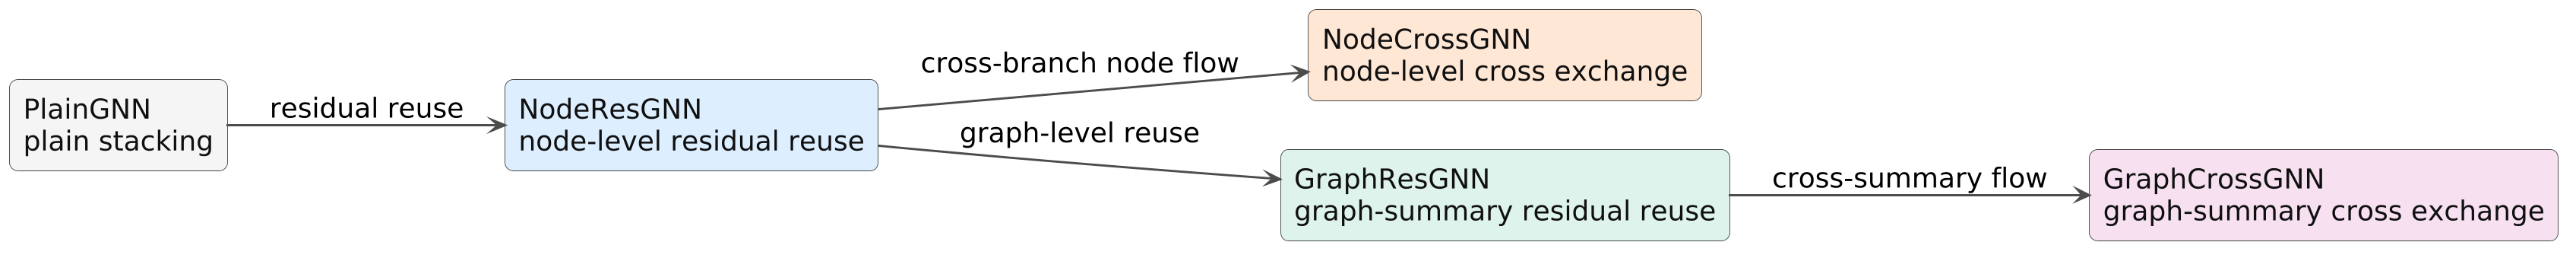
\includegraphics[width=0.98\linewidth]{figures/task_model_comparison.png}
\caption{Main model comparison in this paper. The five architectures differ only in how intermediate node states or graph summaries are reused, which allows a controlled study of residual and cross-residual information flow.}
\label{fig:task_model_comparison}
\end{figure}

\subsection*{Shared message passing and graph-level learning}

Let $\Phi$ denote a message-passing operator. For a chosen backbone, node representations are updated over $L$ layers as
\begin{equation}
\mathbf{h}_i^{(\ell+1)} = \sigma\left(\mathbf{W}^{(\ell)} \cdot \text{AGGREGATE}_{\Phi}\left(\left\{\mathbf{h}_j^{(\ell)} : j \in \mathcal{N}(i)\right\}, \mathbf{h}_i^{(\ell)}\right) + \mathbf{b}^{(\ell)}\right).
\end{equation}
After $L$ layers, a readout function $R$ aggregates node-level representations into a graph embedding
\begin{equation}
\mathbf{h}_{\mathcal{G}} = R\left(\left\{\mathbf{h}_i^{(L)} : i = 1, \ldots, n\right\}\right).
\end{equation}
The classifier produces
\begin{equation}
\hat{\mathbf{y}} = \text{softmax}\left(\mathbf{W}_{\text{clf}} \mathbf{h}_{\mathcal{G}} + \mathbf{b}_{\text{clf}}\right),
\end{equation}
and the model is trained end-to-end by minimizing cross-entropy:
\begin{equation}
\mathcal{L}(\theta) = -\frac{1}{N} \sum_{i=1}^{N} \sum_{c=1}^{C} y_{i,c} \log(\hat{y}_{i,c}).
\end{equation}

\subsection*{CR-GNN architecture family}
\label{sec:model}

CR-GNN is defined as a compact family of graph classification architectures. All variants share the same input projection, stacked message-passing layers, graph-level pooling, and linear classifier; they differ only in how intermediate node states and graph-level summaries are reused across depth and across branches.

\begin{figure}[!htbp]
\centering
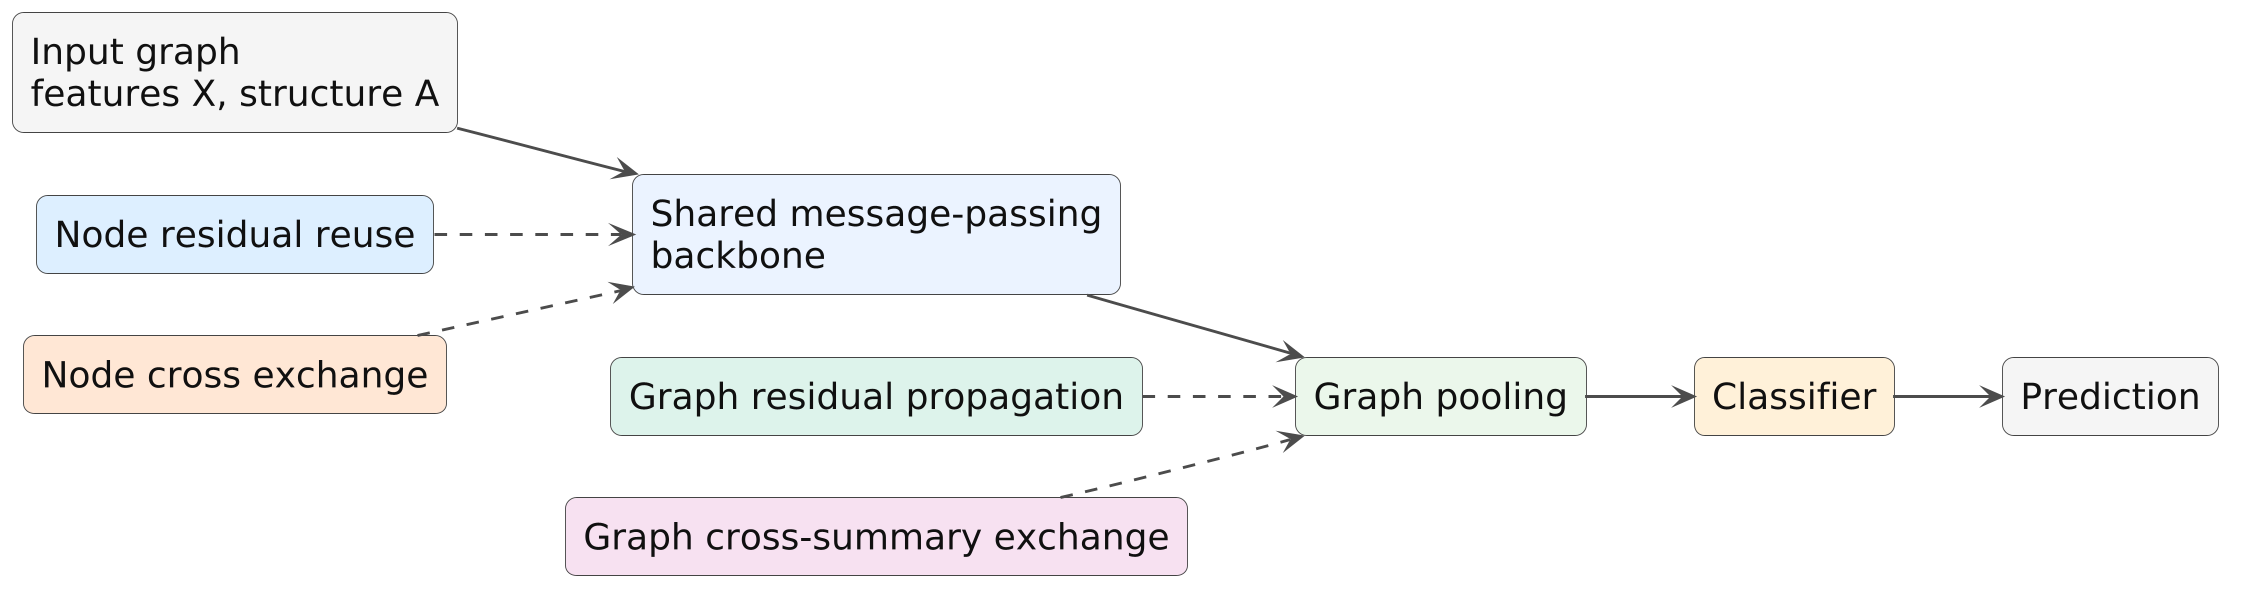
\includegraphics[width=0.98\linewidth]{figures/cr_gnn_schematic.png}
\caption{Schematic view of the CR-GNN pipeline. All models share the same graph-classification backbone, while node-level reuse and graph-level summary reuse define the residual and cross-residual variants.}
\label{fig:crgnn_schematic}
\end{figure}

Let $\mathcal{G}=(\mathcal{V},\mathcal{E})$ be a graph with node feature matrix $\mathbf{X}\in\mathbb{R}^{n\times d_{\mathrm{in}}}$ and adjacency structure $\mathbf{A}$. The model can be instantiated with one of several standard message-passing operators,
\[
\Phi \in \{\mathrm{GCN},\ \mathrm{GAT},\ \mathrm{Graph\mbox{-}Transformer}\},
\]
and reuses the same operator type throughout a model instance. For a hidden width $d$, every branch starts with an input projection
\begin{equation}
\mathbf{H}^{(0)} = \mathrm{ReLU}\!\left(\Phi_{\mathrm{in}}(\mathbf{X}, \mathbf{A})\right),
\end{equation}
followed by $L$ hidden layers and a readout
\begin{equation}
\mathbf{g} = \mathrm{Pool}\!\left(\mathbf{H}^{(L)}\right).
\end{equation}

\subsubsection*{Single-branch and node-level residual variants}

\textbf{PlainGNN.} The plain baseline stacks $L$ copies of the same operator without residual reuse:
\begin{equation}
\mathbf{H}^{(\ell+1)} = \psi\!\left(\mathrm{ReLU}\!\left(\Phi_{\ell}\!\left(\mathbf{H}^{(\ell)}, \mathbf{A}\right)\right)\right).
\end{equation}

\textbf{NodeResGNN.} The first residual variant stores the previous hidden state within the same branch:
\begin{equation}
\mathbf{H}^{(\ell+1)} = \psi\!\left(\mathrm{ReLU}\!\left(\Phi_{\ell}\!\left(\mathbf{H}^{(\ell)} + \mathbf{H}^{(\ell-1)}, \mathbf{A}\right)\right)\right).
\end{equation}

\textbf{NodeCrossGNN.} The node-level cross-residual model maintains two parallel branches with separate input projections:
\begin{align}
\mathbf{H}^{(\ell+1)}_{1} &= \psi\!\left(\mathrm{ReLU}\!\left(\Phi^{(1)}_{\ell}\!\left(\mathbf{H}^{(\ell)}_{1} + \widetilde{\mathbf{H}}^{(\ell)}_{2}, \mathbf{A}\right)\right)\right), \\
\mathbf{H}^{(\ell+1)}_{2} &= \psi\!\left(\mathrm{ReLU}\!\left(\Phi^{(2)}_{\ell}\!\left(\mathbf{H}^{(\ell)}_{2} + \widetilde{\mathbf{H}}^{(\ell)}_{1}, \mathbf{A}\right)\right)\right).
\end{align}
The final node representation is the branch sum
\begin{equation}
\mathbf{H}^{(L)} = \mathbf{H}^{(L)}_{1} + \mathbf{H}^{(L)}_{2}.
\end{equation}

\subsubsection*{Graph-level residual propagation}

\textbf{GraphResGNN.} This variant chains three graph-conditioned blocks:
\begin{equation}
\mathbf{g}^{(t+1)} = B_{t+1}\!\left(\mathbf{X}, \mathbf{A}, \mathbf{g}^{(t)}\right), \quad t \in \{1,2\}.
\end{equation}

\textbf{GraphCrossGNN.} Four blocks are organized as two sequential pairs. Within each stage, the two block outputs are swapped and reused as the next stage's graph-level input:
\begin{align}
(\mathbf{g}^{(t)}_{1}, \mathbf{g}^{(t)}_{2}) &= \left(B_{2t-1}\!\left(\mathbf{X}, \mathbf{A}, \mathbf{g}^{(t-1)}_{1}\right),\ B_{2t}\!\left(\mathbf{X}, \mathbf{A}, \mathbf{g}^{(t-1)}_{2}\right)\right), \\
(\mathbf{g}^{(t+1)}_{1}, \mathbf{g}^{(t+1)}_{2}) &= \left(\mathbf{g}^{(t)}_{2},\ \mathbf{g}^{(t)}_{1}\right).
\end{align}
The final graph embedding is
\begin{equation}
\mathbf{g}_{\mathrm{final}} = \mathbf{g}^{(T)}_{1} + \mathbf{g}^{(T)}_{2}.
\end{equation}

\subsection*{Residual routing mechanisms}

Beyond the architecture family itself, this study evaluates how residual information is injected. Three routing modes are used in the targeted ablations:
\begin{itemize}
    \item \textbf{Learnable routing}: dense residual injection modulated by an adaptive gate.
    \item \textbf{Top-k routing}: only the strongest residual channels are retained before injection.
    \item \textbf{Sparse routing}: weak residual coefficients are suppressed, leaving a filtered residual path.
\end{itemize}
These routing modes are not used to redefine the core architecture family. Instead, they form a mechanism layer on top of selected residual and cross-residual targets in the experimental design.

\subsection*{Datasets}
\label{sec:datasets}

To test the proposed architecture in a biologically meaningful setting, the benchmarks are organized into a unified two-layer package.

The main biological benchmark consists of PROTEINS, DD, and ENZYMES \cite{fey2019fast,morris2020tudataset}. The supplementary robustness package consists of MUTAG, AIDS, and Mutagenicity. This organization keeps the main biological claim centered on protein-oriented datasets while still testing structural robustness on additional molecular graphs.

\paragraph{PROTEINS}
PROTEINS contains graph representations of proteins, where nodes denote secondary structure elements and edges encode neighborhood relations between them. The task is binary graph classification. The dataset contains 1,113 graphs, 2 classes, and 3 input features per node.

\paragraph{DD}
DD is a protein structure dataset in which each graph corresponds to a protein and nodes represent amino acids or structure-related units linked by proximity-derived edges. The task is binary classification. DD contains 1,178 graphs, 2 classes, and 89 input features.

\paragraph{ENZYMES}
ENZYMES is a 6-class enzyme classification benchmark with 600 graphs and 3 input features. It preserves an enzyme-oriented biological interpretation while remaining directly comparable to the other graph classification benchmarks in the study.

\begin{table*}[!t]
\centering
\small
\caption{Unified summary of the main biological benchmark package.}
\label{tab:dataset_main_package}
\setlength{\tabcolsep}{4pt}
\begin{tabular}{l l c c c c l}
\toprule
Dataset & Split & \#Graphs & \#Cls. & Feat. & Avg. N / E & Role \\
\midrule
PROTEINS & 5-fold CV + val & 1113 & 2 & 3 & 39.1 / 72.8 & main \\
DD & 5-fold CV + val & 1178 & 2 & 89 & 284.3 / 715.7 & main \\
ENZYMES & 5-fold CV + val & 600 & 6 & 3 & 32.6 / 62.1 & main \\
\bottomrule
\end{tabular}
\end{table*}

\begin{table*}[!t]
\centering
\small
\caption{Supplementary robustness datasets retained outside the core biological narrative.}
\label{tab:dataset_supp_package}
\setlength{\tabcolsep}{4pt}
\begin{tabular}{l l c c c c l}
\toprule
Dataset & Split & \#Graphs & \#Cls. & Feat. & Avg. N / E & Role \\
\midrule
MUTAG & 5-fold CV + val & 188 & 2 & 7 & 17.9 / 19.8 & supp. \\
AIDS & 5-fold CV + val & 2000 & 2 & 38 & 15.7 / 16.2 & supp. \\
Mutagenicity & 5-fold CV + val & 4337 & 2 & 14 & 30.0 / 30.6 & supp. \\
\bottomrule
\end{tabular}
\end{table*}


All active datasets are used through a unified benchmark interface \cite{fey2019fast,morris2020tudataset}. We keep preprocessing intentionally light and do not introduce task-specific feature engineering, graph augmentation, or edge redesign in the final protocol.

All reported results follow the same stratified two-stage evaluation design:
\begin{itemize}
    \item \textbf{Outer evaluation}: stratified 5-fold cross-validation at the graph level
    \item \textbf{Inner validation}: a stratified validation subset sampled from the training fold with validation ratio 0.1
\end{itemize}

The primary evaluation metric is graph classification accuracy on the held-out test fold. For fold $k$ with test set $\mathcal{T}_k$, the fold accuracy is
\begin{equation}
\mathrm{Acc}_k = \frac{1}{|\mathcal{T}_k|}\sum_{(\mathcal{G}_i,y_i)\in\mathcal{T}_k}\mathbf{1}\!\left[\hat{y}_i = y_i\right].
\end{equation}
Across the five folds, we report the mean accuracy
\begin{equation}
\overline{\mathrm{Acc}} = \frac{1}{5}\sum_{k=1}^{5}\mathrm{Acc}_k
\end{equation}
and the corresponding standard deviation
\begin{equation}
\sigma_{\mathrm{Acc}} = \sqrt{\frac{1}{5}\sum_{k=1}^{5}\left(\mathrm{Acc}_k-\overline{\mathrm{Acc}}\right)^2 }.
\end{equation}

\subsection*{Compared methods and backbone operators}

The full paper-facing benchmark compares nine methods. The CR-GNN family contains five models: PlainGNN, NodeResGNN, NodeCrossGNN, GraphResGNN, and GraphCrossGNN. Four external baselines are also included in the benchmark package: GraphSAGEBaseline, GINBaseline, JKNetBaseline, and APPNPBaseline.

Each method is evaluated under four message-passing operators:
\begin{itemize}
    \item \textbf{GCNConv}
    \item \textbf{GATConv}
    \item \textbf{GINConv}
    \item \textbf{SAGEConv}
\end{itemize}

\subsection*{Training configuration and implementation details}

All reported runs follow the same versioned experimental workflow, with \texttt{V3} as the active paper-facing source. The recommended workflow entry is \texttt{py/run\_final\_v3\_pipeline.py}, and the associated outputs are stored in \texttt{logs/V3}, \texttt{records/V3}, and \texttt{runs/V3}. Preprocessing is intentionally light, and the final protocol does not add task-specific feature engineering, graph augmentation, or custom edge redesign.

\subsection*{Evaluation metrics and statistical reporting}

The primary metric is graph classification accuracy on the held-out test fold. Main benchmark and targeted ablation results are reported as five-fold mean accuracy with standard deviation. In the final paper, the five-fold \texttt{V3} experiments are treated as the main confirmatory evidence, while older single-fold parameter scans are used only as supporting exploratory analyses.
